\chapter{Visualization of \gls{DICOM} images}

\section{Display (brightness) standarization}
\begin{itemize}
\item To ensure \emph{visual consistency}, that image looks the same
  regardless of which monitor or display device it's viewed on.
\item This is achieved through the \gls{GSDF} \cite{DICOM_GSDF}, that
  expresses the \popup{luminance}{Luminosity, usually measures in
    candelas per square meter
    (\popup{cd}{Candelas.}/\popup{m}{Meter.}$^2$).} that a display
  should produce as a function of the pixels values. Thus, the
  luminance that a pixel with with \popup{value}{P-Value in terms of
    the standard notation.} $x$ (the should have is
  \begin{equation}
    L(j) = \exp\left(\sum_{i=0}^{9}a_i\big(\ln j(x)\big)^i\right),
  \end{equation}
  where
  \begin{center}
  \begin{tabular}{l}
    $a_0 = -1.3011877$, \\
    $a_1 = -2.5840191E-2$, \\
    $a_2 = 8.0242636E-2$, \\
    $a_3 = -1.0320229E-1$, \\
    $a_4 = 1.3646699E-1$, \\
  \end{tabular}
  \begin{tabular}{l}
    $a_5 = 2.8745620E-2$, \\
    $a_6 = -2.5468404E-2$,\\
    $a_7 = -3.1978977E-3$, \\
    $a_8 = 1.2992634E-4$, \\
    $a_9 = 1.3635334E-3$,
  \end{tabular}
  \end{center}
  and where
  \begin{equation}
    j(x) = j_{\text{min}} + \frac{j_{\text{max}} - j_{\text{min}}}{n(x)},
  \end{equation}
  being $j_{\text{min}}$ and $j_{\text{max}}$ are the \popup{minimum
    and maximum \gls{JND} index within the luminance range of the
    display}{That a normal human being can recognize in the display
    which is being standardized.}, and where
  \begin{equation}
    n(x) = \frac{x}{2^N-1},
  \end{equation}
  where $N$ is thee number of bits/pixel.
\end{itemize}

\begin{figure}[H]
  \vspace{-0ex}
  \centering
  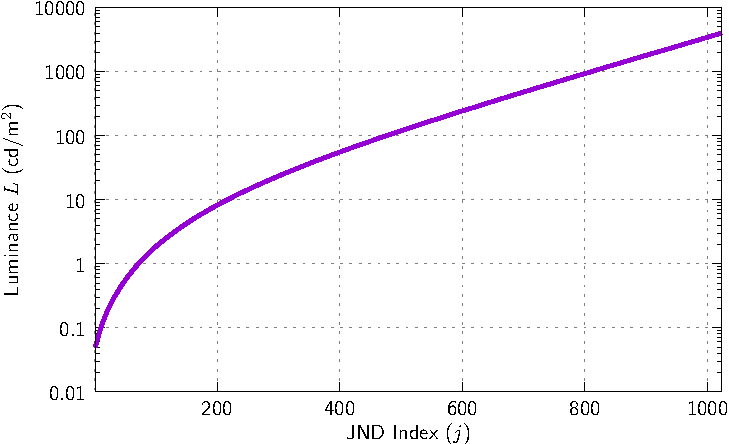
\includegraphics[width=0.7\textwidth]{GSDF}
  \caption{\gls{GSDF} used in \gls{DICOM}.}
  \label{fig:GSDF}
\end{figure}

\begin{itemize}
\item This way, equal steps in pixel values correspond to equal
  perceptual differences (\glspl{JND}).
\item In other words, a \popup{step}{An increment in one in the
  integer value of ...} in \gls{JND} corresponds as the smallest
  brightness change detectable by the average human eye.
\end{itemize}
